\section{Vorbereitungsfragen}
\subsection{Erläutern sie die Begriffe Wärmedurchgangskoeffizient, Wärmeübergangswiderstand, Wärmeleitfähigkeit und Wärmestrahlung}

\begin{itemize}
\item Wärmedurchgang ist der Wärmeübergang von einem Fluid durch eine Wand auf ein anderes Fluid und wird durch den Wärmedurchgangskoeffizienten beschrieben. Der Wärmedurchgangskoeffizient ist ein stoffspezifischer Wert und wird nach \autoref{eq:230523_Wärmedurchgangskoeff} berechnet. 
 
\begin{equation}
	\centering
	u=\frac{1}{R_{si}+\sum_{i=1}^N \frac{d_i}{\lambda_i}+R_{se}}
	\label{eq:230523_Wärmedurchgangskoeff}
\end{equation}

\item Der Wärmeübergangswiderstand $R_s$ beschreibt die Wärmeübertragung zwischen einem Festkörper und einem Fluid. Er ist als der Kehrwert der Wärmeübergangskoeffizienten definiert.

\item Die Wärmeleitfähigkeit $\lambda$ ist die Stoffeigenschaft eines Materials einen Wärmestrom zu leiten. Sie gibt Aussage darüber wie sich Wärme in einem Stoff ausbreitet und ist auch stoffspezifisch.

\item Wärmestrahlung ist eine Art der Wärmeübertragung durch elektromagnetische Wellen im infraroten Bereich.

\end{itemize}




\subsection{Skizzieren sie den Temperaturverlauf und den Wärmestrom durch eine mehrschichtige Wand. Der Wärmestrom verläuft in Richtung des Temperatur gefälles.}
\begin{figure}[H]
	\centering
	\begin{subfigure}[c]{0.303\textwidth}
		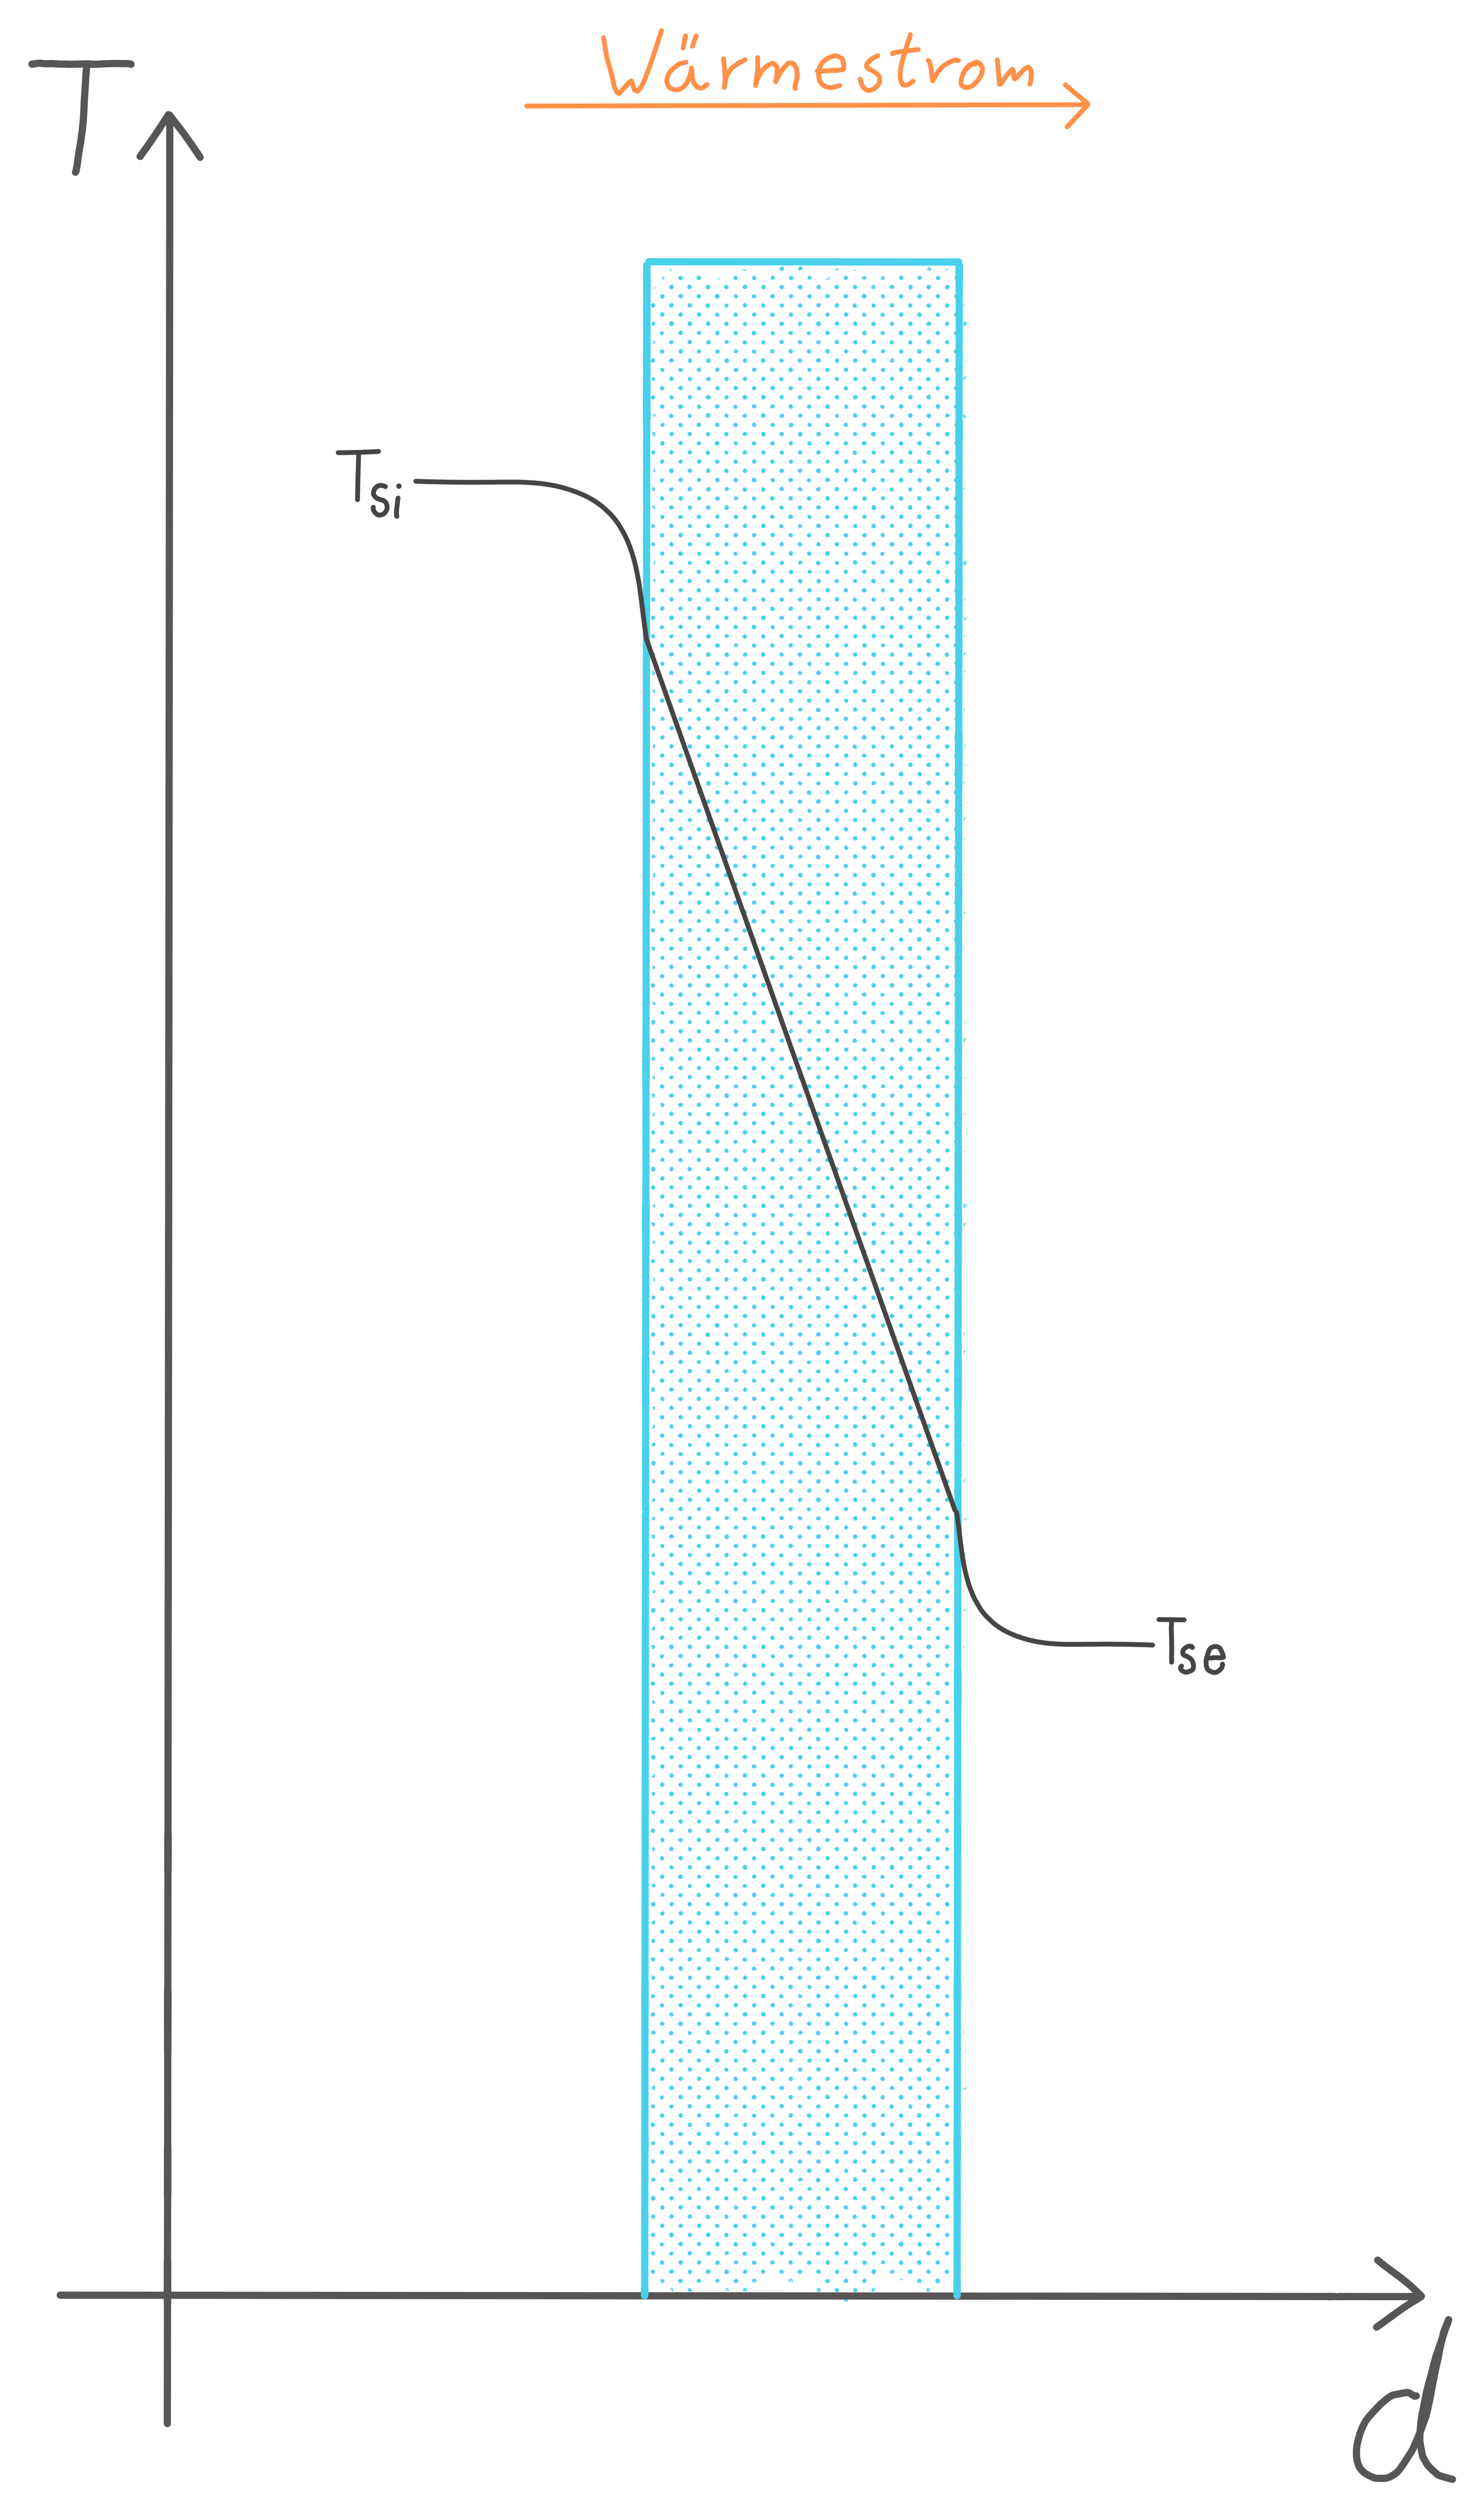
\includegraphics[width=\textwidth]{Abbildungen/einschichtig.png}
		\caption{Einschichtige Wand}
	\end{subfigure}
	\begin{subfigure}[c]{0.497\textwidth}
		\includegraphics[width=\textwidth]{Abbildungen/mehrschichtig.png}
		\caption{Mehrschichtige Wand}
	\end{subfigure}
	\caption{Skizzen der Temperaturverläufe und Wärmeströme verschiedener Wände}
	\label{fig:230515_Temp-verlauf}
\end{figure}
\subsection{Was sagt der Wärmedurchgangskoeffizient aus?}
Der Wärmedurchgangskoeffizient U ist eine Kennzahl, die den Wärmedurchgang durch einen Bauteil oder eine Bauteilschicht beschreibt. 
Er gibt an, wie viel Wärme pro Zeiteinheit und pro Fläche durch das Bauteil hindurchgeht, wenn ein Temperaturunterschied zwischen den beiden Seiten des Bauteils herrscht.
Der U-Wert wird in der Einheit $$\frac{W}{m^2 \cdot K}$$ angegeben. Je niedriger der U-Wert ist, desto besser ist die Wärmedämmung des Bauteils. 
Ein niedriger U-Wert bedeutet, dass weniger Wärmeenergie verloren geht und das Bauteil effizienter dämmt.
Der U-Wert berücksichtigt verschiedene Faktoren wie die Materialien, die Dicke der Bauteilschichten, eventuelle Luftspalten und Wärmebrücken. 
Er wird verwendet, um den Energieverbrauch von Gebäuden zu berechnen, die Effizienz von Wärmedämmmaßnahmen zu bewerten und den Wärmeschutz von Bauteilen zu beurteilen.
\subsection{Wie sollte eine Wand beschaffen sein, damit Temperaturschwankungen auf der Außenseite sich innen möglichst wenig auswirken?}
Die Physikalisch simpelste Lösung ist es die Wand massiver zu machen, wodurch die Trägheit des Systems erhöht wird.
bei einer hohen Trägheit verhält sich das System wie ein Tiefpassfilter, langsame Temperaturschwankungen sind auf der Innenseite jedoch immernoch merkbar.
Die bessere Lösung ist es, die Wandkomposition zu verändern und eine bessere Dämmung einzubauen.
Das kann durch Mehrschichten und/oder interne Luftschichten erzielt werden.
Dies hat den Effekt, dass die Innentemperaturen besser gehalten werden und leichter geregelt werden können.

\subsection{Berechnen Sie den Gesamtwärmedurchgangswiderstand für die gegebenen mehrschichtigen Wände (Messreihe 2 Wandaufbau 1 und 2) mit Tabellenwerten aus der einschlägigen Literatur}
\begin{itemize}
\item Grundlegende Gleichung zur Berechnung ist \autoref*{eq:230523_Wärmedurchgangskoeff}
\item $$R_{si}=0,13\frac{m^2 \cdot K}{W}$$ und $$R_{se}=0,04\frac{m^2 \cdot K}{W}$$ sind gegebene Werte
\item lambda-Werte für die Baustoffe immer den schlechtesten Wert angenommen(siehe Excel) aus entsprechenden Normen
\item lamda-Werte für Holz\cite[S.20]{lamda-holz-luft} und Luft\cite[S. 15]{lamda-holz-luft} aus DIN EN ISO 10456:2010-05
\item lamda-Wert für XPS \cite[S.23]{lamda-xps} aus DIN 4108-4:2020-11
\item $$U_{Wand 1}=1,6362 \frac{W}{m^2 \cdot K}$$
\item $$U_{Wand 2}=1,3311 \frac{W}{m^2 \cdot K}$$
\end{itemize}


\subsection{Überlegen Sie, warum es zu Unterschieden zwischen Ihren nach Norm und nach Messungen berechneten U-Werten kommen kann.}